\documentclass[11pt, a4paper, notitlepage]{report}
\usepackage[dvips]{graphicx,color,rotating}
\usepackage{polski}
\usepackage[utf8]{inputenc}
\usepackage{pstricks}
\usepackage{lipsum}
\usepackage{titling}
\usepackage{appendix}
\usepackage{hyperref}
\usepackage{spverbatim}

\pretitle{
	\begin{center}
		
\includegraphics[width=40pt,height=40pt]{graphics/znak_pk} \\
		 \Huge\bfseries}
\posttitle{\par\end{center}\vskip 0.5em}
\preauthor{\begin{center} \Large  SI  \\  \LARGE\ttfamily}
\postauthor{ \end{center}}
\predate{\par\large\centering}
\postdate{\par}

\pagestyle{headings}

\author{Krzysztof \textsc{Michalski} \\ Rafał \textsc{Pokrywka} }

\title{\textbf{Sample usage of NLP with deep learning}}
\date{18.06.2021}

\pagenumbering{roman}

\begin{document}
\clearpage\maketitle
\thispagestyle{empty}
\begin{abstract}
	W tym projekcie zajęliśmy się analizą sentymentu tekstu. Naszym zbiorem danych były posty z Twittera: \href{https://www.kaggle.com/crowdflower/twitter-airline-sentiment}{Twitter US Airline Sentiment}. Każdy z tych postów zawierał jakąś opinię o linii lotniczej, oraz etykiety określające sentyment.
	Naszym celem było stworzenie klasyfikatora pozwalającego określić czy dany tekst był opinią pozytywną, neutralną, czy negatywną. Najlepszy okazał się model sieci neuronowej z 3 warstwami, posiadający 50 jednostek LSTM. Uzyskał on dokładność około 81\% względem zbioru testowego. \\

	Repozytorium: \href{https://github.com/ravkr/SI-NLP}{https://github.com/ravkr/SI-NLP}
\end{abstract}

\clearpage \tableofcontents
\thispagestyle{empty}

\setcounter{page}{1}

\chapter{Wprowadzenie}
\pagenumbering{arabic}
W naszym projekcie użyliśmy zbioru danych \href{https://www.kaggle.com/crowdflower/twitter-airline-sentiment}{Twitter US Airline Sentiment}. Są to tweety skierowane do linii lotniczych, najczęściej z opinią o nich. Dane znajdują się w pliku csv zawierającym 14845 wierszy i 15 kolumn. Do przeprowadzenia analizy sentymentu użyjemy wyłącznie tekstu oraz informacji o pozytywności danego posta, więc oczyściliśmy dane, usuwając wszystkie inne kolumny. Dodatkowo usunęliśmy też znaki cudzysłowu.
\\
Rozkład rodzajów opinii był następujący:
\begin{itemize}
    \item positive - 2363 - 16,1 \%
    \item neutral - 3099 - 21,2 \%
    \item negative - 9178 - 62,7 \%
\end{itemize}
Widać, że przeważała ilość opinii negatywnych - jest ich więcej niż wszystkich pozostałych. Trzeba o tym pamiętać podczas tworzenia klasyfikatorów, ponieważ nawet zwracanie wyniku "negative" za każdym razem dałoby prawidłową odpowiedź w aż 62,7 \% przypadków.

\section{Opis problemu}
Analiza sentymentu - jest to użycie NLP (przetwarzanie języka naturalnego) i analizy tekstu, w celu określania znaczenia tekstu, najczęściej określenia, czy jest on nacechowany pozytywnie czy negatywnie.
\\
W wybranym przez nas zbiorze danych teksty są oznaczone jako pozytywne, negatywne lub neutralne. Oznacza to, że będziemy wykonywać klasyfikację wieloklasową. Dla potrzeb sieci neuronowych, wykorzystamy kodowanie gorącojedynkowe.

\section{Analiza tekstu}
W ramach oczyszczania danych tekstowych z wykorzystaniem biblioteki fastText, zebraliśmy kilka informacji pokazujących charakterystykę tekstu zawartego w tweetach. Po oczyszczeniu tweetów z elementów, które nie niosą znaczenia (na przykład często występujące słowa) mamy następujące informacje:
\begin{itemize}
    \item Średnia ilość słów występująca w tweecie - 10.05 słów
    \item Procent słów występujących w tweecie po oczyszczeniu - 56.65 \%
    \item Puste wektory znaczeniowe uzupełniające tekst:
    \begin{itemize}
    \item  przy stałej długości 6 słów - 0.44 wektora na tweet, ucięte słowa - 4.49 słowa na tweet
    \item  przy stałej długości 10 słów - 1.73 wektora na tweet, ucięte słowa - 1.78 słowa na tweet
    \item  przy stałej długości 20 słów - 9.94 wektora na tweet, ucięte słowa - 0.002 słowa na tweet
    \end{itemize}
\end{itemize}

\begin{center}
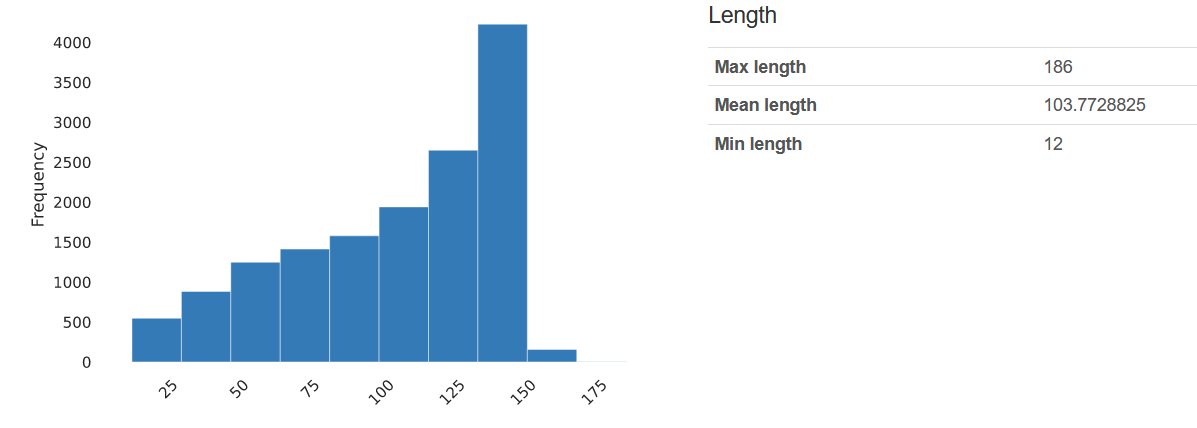
\includegraphics[width=350pt]{graphics/analiza_dlugosci_tekstu.png}
\end{center}

W naszym zbiorze danych najwięcej jest "długich" tekstów, tzn. mających 130-140 bajtów - około 4 tysięcy rekordów (27 \%). Wynika to z ograniczenia długości postów na Twitterze to 140 znaków. Niektóre teksty mają ponad 140 bajtów (maksymalnie 186), ponieważ znaki diakretyczne, emoji itp. mogą zajmować więcej niż jeden bajt na znak. Średnia długość tweeta to 104 bajty. Krótkich tweetów jest najmniej, ponieważ w np. 25 znakach ciężko jest zmieścić coś więcej niż nazwę linii lotniczej i więcej niż kilka słów. \\
Przy takich krótkich tekstach (np. "@united thanks") analiza sentymentu może dawać słabe rezultaty, ponieważ ciężko jest z jednego słowa wywnioskować co autor miał na myśli - mogło to być "podziękowanie" za opóźnienie, a mogło to być podziękowanie za odpowiedź na inną wiadomość.



\begin{center}
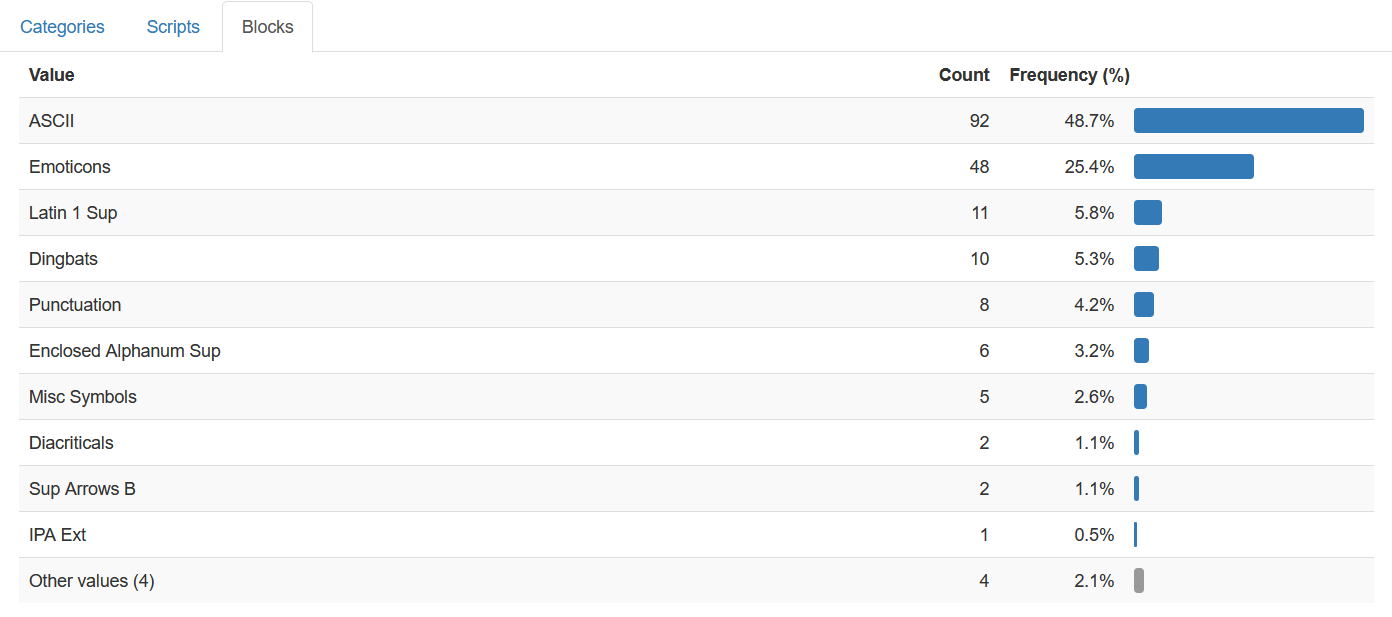
\includegraphics[width=350pt]{graphics/analiza_rodzajow_znakow.png}
\end{center}
Najwięcej znaków w tekstach, to znaki ASCII (48,7 \%). Dużą część stanowią też znaki emoji (25,4 \%) - jest ich dużo w stosunku do znaków ASCII, ponieważ na Twitterze obowiązuje limit znaków i wiele słów jest zastępowanych znakami różnych emotikon, m.in emoji. Dodatkowe litery (np. z diakrytykami) i znaki ozdobne (np. emotikony inne niż emoji) stanowią kolejno 5,8 \% i 5,3 \% wszystkich znaków. Interpunkcja to 4,2 \%.


\chapter{Opis metody}
\section{Wprowadzenie teoretyczne}
W celu rozwiązania zadania wykorzystaliśmy kilka różnych bibliotek Pythona:
\\ \\ {\bf fastText} - jest to biblioteka stworzona przez Facebooka. Biblioteka ta zawiera wytrenowane wcześniej modele dla języka angielskiego, przez co nie trzeba (chociaż można) dodatkowo przeprowadzać procesu uczenia. Biblioteka wymaga osobnych plików treningowych i testowych w formacie txt. Każda linijka jest kolejnym rekordem, a etykiety danych oznacza się poprzez {\bf \_\_label\_\_} przed słowem z etykietą, przykładowo: {\bf \_\_label\_\_negative}.
\\ \\

{\bf Keras} - z tej biblioteki będziemy korzystać w celu stworzenia następujących rodzajów warstw sieci neuronowej:

\begin{itemize}
    \item {\bf Warstwa gęsta} (ang. dense layer) - warstwa, której wszystkie wejścia są połączone ze wszystkimi możliwymi wyjściami warstwy poprzedniej.
    \item {\bf Warstwa rekurencyjna} - warstwa, w której dane przekazywane są nie tylko z wyjścia neuronów z poprzedniej do obecnej warstwy, ale również istnieją połączenia pomiędzy kolejnymi neuronami w tej samej warstwie. Sieci neuronowe zawierające warstwy rekurencyjne pozwalają nie tylko na przwidywanie wyników z pojedynczych rekordów (np. zdjęcie lub słowo), ale również z sekwencji danych (np. film lub zdanie). Ponieważ dane wejściowe do neuronów zawierają również wyniki operacji z poprzednich neuronów, to przewidywania takiej sieci mogą być dokładniejsze. Przykładowo w zdaniach "nie nudziłem się" i "nie jest super", słowo "nie" za pierwszym razem zmienia negatywne znaczenie tesktu na pozytywne, a za drugim z pozytywnego na negatywne. Używając rekurencyjnej sieci neuronowej (RNN - ang. recurrent neural network) podczas analizy słów "nudziłem się" i "jest super" słowo "nie" jest już zawarte w wektorze danych wejściowych. Klasyczne sieci rekurencyjne przy dużej ilości warstw zaczynają mieć problemy podczas uczenia, spowodowane zanikającym gradientem. Najwyższe warstwy uczą się względnie szybko, a te najniższe, początkowe, prawie w ogóle. Aby rozwiązać ten problem stworzono neurony z pamięcią, przekazujące i zapamiętujące część poprzedniego wyniku. Najczęściej są to jednostki rekurencyjne jednego z dwóch typów:
    \begin{itemize}
            \item {\bf Jednostki rekurencyjne LSTM} (ang. Long short-term memory) - każda jednostka posiada trzy wejścia i dwa wyjścia. Jedno z wejść to dane z wyjścia poprzedniej warstwy sieci, drugie wejście to wynikowe wyjście z poprzedniej jednostki w tej samej warstwie, a trzecie wejście to "pamięć" poprzedniej jednostki.\\
        Działanie tej jednostki przebiega następująco:
        \begin{itemize}
            \item {\bf Bramka zapominająca} - Na podstawie wejścia pierwszego i drugiego obliczane jest ile danych z wejścia trzeciego powinno zostać zapamiętanych i przekazanych dalej.
            \item {\bf Bramka wejściowa} - Na podstawie wejścia pierwszego i drugiego obliczane jest ile danych z tych wejść zostanie dodane do pamięci obecnej jednostki. Wynik dodawania zostaje przekazany później do kolejnej jednostki.
            \item {\bf Bramka wyjściowa} - Na podstawie wejścia pierwszego i drugiego oraz pamięci obecnej jednostki, wyliczane jest wyjście tej jednostki.
        \end{itemize}

        \begin{center}
        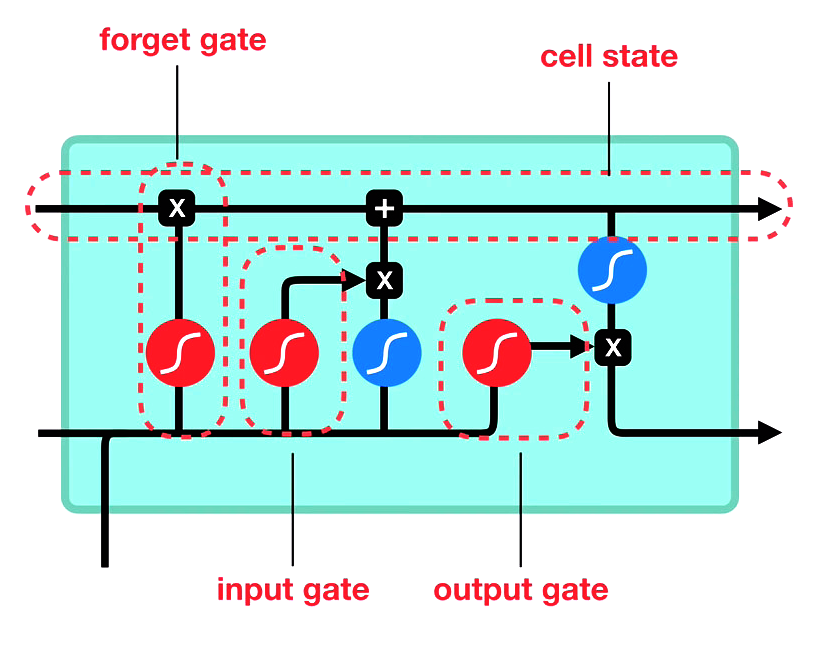
\includegraphics[width=300pt]{graphics/LSTM gate.png}
        \end{center}

        \\
        \item {\bf Jednostki rekurencyjne GRU} (ang. Gated recurrent unit) - działanie tej jednostki jest podobne do LSTM, jednak ma prostszą budowę. Każda jednostka posiada dwa wejścia (zamiast trzech): pamięć poprzedniej jednostki i wyjście z poprzedniej warstwy, oraz tylko jedno wyjście ("pamięć" tej jednostki). W jej budowę wchodzi bramka resetująca, oraz bramka aktualizująca.

        Działanie tej jednostki przebiega następująco:
        \begin{itemize}
            \item {\bf Bramka resetująca} - Na podstawie obydwu wejść obliczane jest ile danych ze stanu poprzedniej jednostki powinno zostać zapomniane.
            \item {\bf Bramka aktualizująca} - Na podstawie obydwu wejść obliczana jest część danych która zostanie dodana (z wejścia z poprzedniej warstwy) i część danych która zostanie zapomniana (ze stanu poprzedniej jednostki). Po dodaniu do siebie części pozostawionej z pamięci poprzedniej jednostki i części wejścia obecnej jednostki, na wyjściu pojawia się nowy stan pamięci tej jednostki.
        \end{itemize}

        \begin{center}
        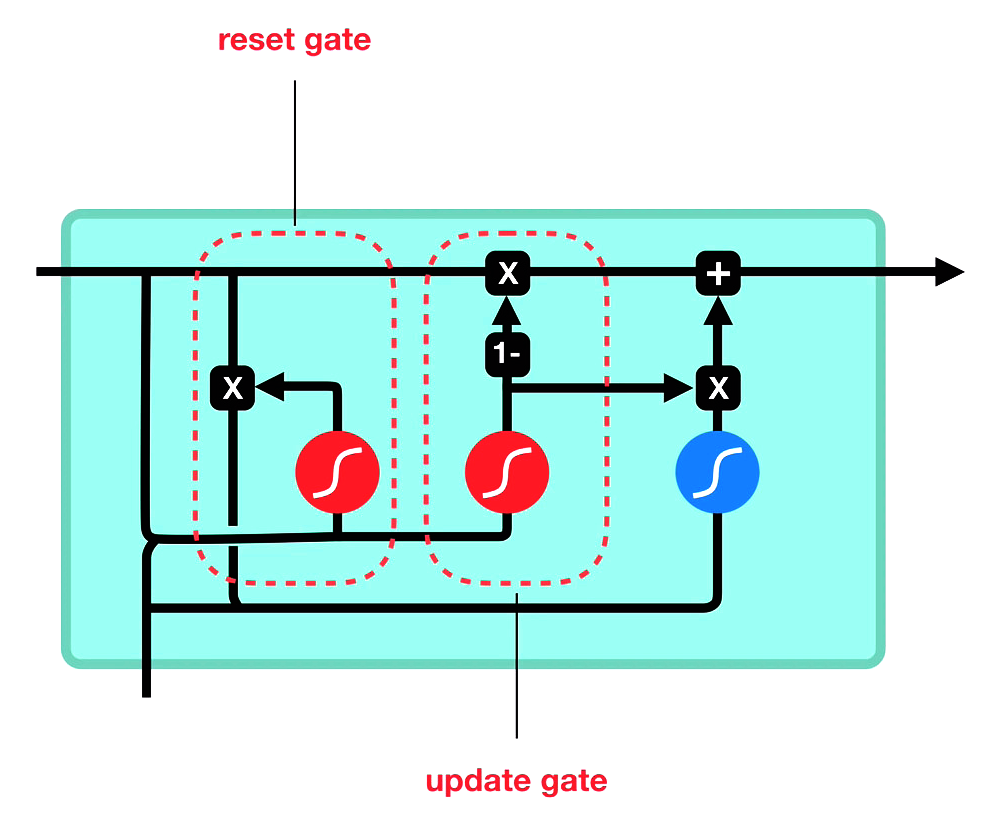
\includegraphics[width=300pt]{graphics/GRU gate.png}
        \end{center}
    \end{itemize}
\end{itemize}

    \begin{center}
    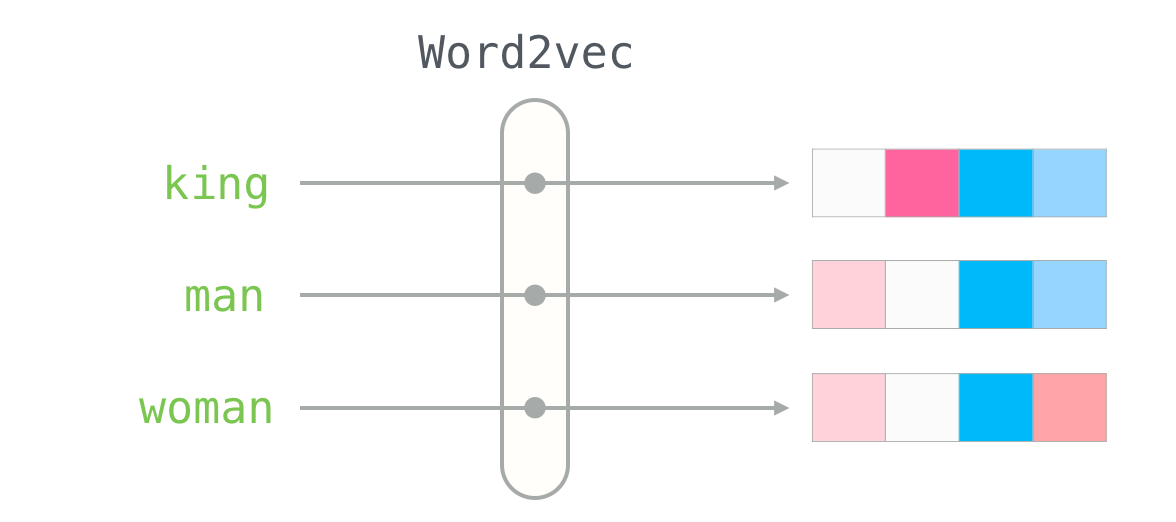
\includegraphics[width=300pt]{graphics/word2vec.png}
    \end{center}

{\bf word2vec} - technika kodowania słów w postaci wektorów liczb zmiennoprzecinkowych w przestrzeni znaczeniowej słów. Wykorzystuje się w niej sieci neuronowe trenowane na dużych korpusach tekstowych. Wytrenowany model pozwala na przykład wykrywać synonimy wśród słów.
\\ \\
Wektory te nazywane są po angiesku word embedding. Mają one taką cechę, że miara odległości cosinusowej pomiędzy tymi wektorami - czyli cosinusa kąta pomiędzy nimi - jest proporcjonalna do poziomu podobieństwa znaczeniowego pomiędzy słowami reprezentowanymi przez te wektory. Posiadają one również ciekawą cechę pozwalającą sumować i odejmować znaczenia słów na przykład:
\\ \\
król - mężczyzna + kobieta = królowa
\\ \\
{\bf n-gram} - model językowy, który służy do kodowania tekstów. Polega on na tym, że dana sekwencja słów jest dzielona na podciągi słów o określonej długości, czyli właśnie n-gramów. N-gram o długości jeden to zbiór słów występujących w tekście, o długości 2 to pary sąsiednich słów danego tekstu i analogicznie dla dłuższych n-gramów. Pozwalają one na ekstrakcję cech z tekstu, zamieniając go na kolumny reprezentujące obecność w danym tekście danego ciągu słów.

\section{Badania symulacyjne}
\subsection{Model z użyciem n-gramów z biblioteki fastText}
Na początku przetestowaliśmy wbudowany algorytm do uczenia nadzorowanego z wykorzystaniem n-gramów z biblioteki fastText. Wczytaliśmy zatem dane treningowe i testowe z osobnych plików (zbiór został podzielony wcześniej ręcznie) i wytrenowaliśmy modele na kilka różnych sposobów.
Sprawdziliśmy różne wielkości n-gramów (od 1 do 4), oraz różne ilości epok uczenia (od 5 do 25, z krokiem 5). Poniżej na wykresach porównanie uzyskanych rezultatów z użyciem metryki dokładności klasyfikacji dla każdej klasy oddzielnie oraz wszystkich razem dla danych ze zbioru testowego:

\begin{center}
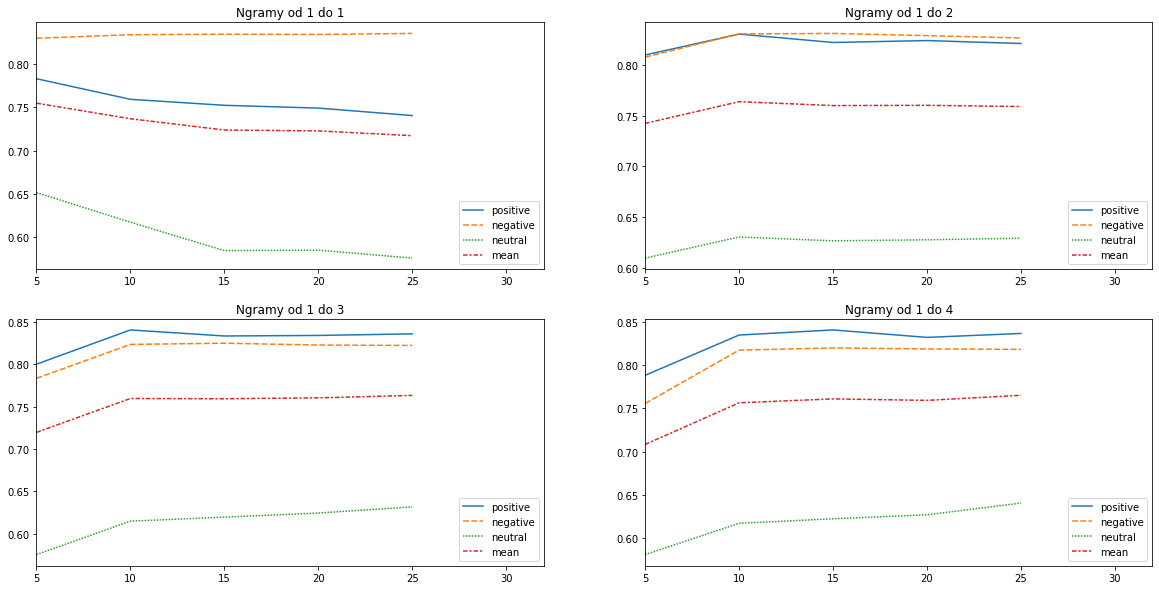
\includegraphics[width=350pt]{graphics/ngramy.png}
\end{center}

Na wykresach jest przedstawiona precyzja przewidywań dla różnych rodzajów tesktu (pozytywny, neutralny, negatywny), oraz średnia z prezycji tych przewidywań.
Można odczytać, że najlepsze wyniki dają n-gramy od 1 do 3 i od 1 do 4, przy 25 epokach uczenia.
Jednak podobne efekty daje też uczenie z n-gramami od 1 do 2, już nawet przy 10 epokach. Zależnie od potrzeb, można skrócić czas uczenia używając właśnie tego sposobu. Prawdopodobnie przy większej ilości tekstów i słów, różnice mogłyby być większe.

Precyzja na poziomie ~75 \% oznacza, że przewidywanie działa prawidłowo, ponieważ przy klasyfikacji naiwnym klasyfikatorem Bayesa R-0 otrzymalibyśmy dokładność 62,7 \%.

\subsection{Przygotowanie danych dla modelu sieci neuronowej}

Następnie chcieliśmy sprawdzić modele sieci neuronowych. W tym celu pobraliśmy (wbudowaną metodą) model języka angielskiego oraz wczytaliśmy dane z pliku (całość w jednym), a następnie podzieliliśmy na zbiór testowy (20 \%) i treningowy (80 \%).
W ramach czyszczenia danych usunęliśmy znaki niewystępujące w języku angielskim oraz słowa, które zbyt często występują w języku angielskim i nie niosą żadnego znaczenia - tak zwane stopwords.
\\
Dla uzyskanych w ten sposób słów przeprowadziliśmy konwersję używając wektorów znaczeniowych słów typu word2vec z biblioteki fastText - dla każdego słowa jest to wektor 300 cech (liczb zmiennioprzecinkowych) w przestrzeni znaczeniowej słów. Sieci rekurencyjne wymagają, żeby każdy przykład składał się z takiej samej liczby elementów. Z tego względu ponieważ tweety zawierają różną liczbę słów - znormalizowaliśmy ich ilość tworząc zbiory z 6, 10 i 20 słowami na tweet (ucinając nadmiarowe słowa i wypełniając brakujące wektorem zawierającym zera).
\\
Ze względu na bardzo duże zużycie pamięci przez model fastText - około 10 GB pamięci RAM - przed trenowaniem sieci zapisaliśmy zbiór testowy i treningowy do plików binarnych biblioteki NumPy.
\\
W kolejnym kroku zamieniliśmy etykiety tekstowe, na wartości liczbowe zakodowane w postaci wektorów one hot encoding typu (0,0,1) zamiast słów 'negative', 'neutral' i 'positive'.

\subsection{Sieci neuronowe z jednostkami LSTM i GRU}

Próbujemy teraz stworzyć sieci neuronowe z kilkoma warstwami, które będą miały za zadanie rozpoznać sentyment tekstu. Jako dane wejściowe używamy przygotowanych wcześniej wektorów liczbowych, utworzonych na podstawie tekstów. Na początku zbudowaliśmy następujące sieci 3 warstwowe:
\\ \\
\begin{center}
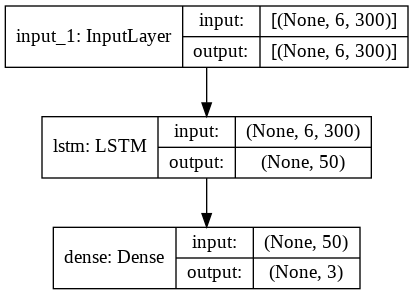
\includegraphics[width=115pt]{graphics/model_LSTM_3_warstwy_6.png}
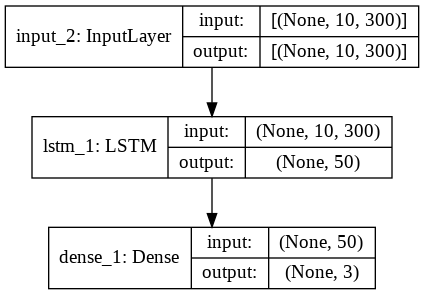
\includegraphics[width=115pt]{graphics/model_LSTM_3_warstwy_10.png}
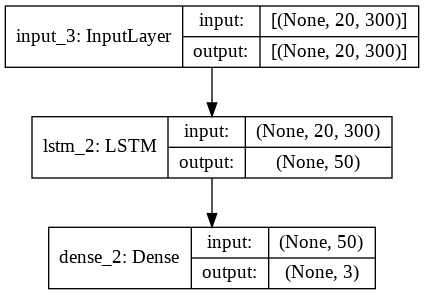
\includegraphics[width=115pt]{graphics/model_LSTM_3_warstwy_20.png}
\end{center}
Sieci te różnią się obsługiwaną ilością słów na tweet. Każde słowo jest reprezentowane w postaci wektora znaczeniowego zawierającego 300 liczb zmiennoprzecinkowych (stąd wejściem do sieci jest macierz o wymiarach liczba\_przykładów\_uczących x liczba\_słów x 300). Każda sieć posiada warstwę rekurencyjną LSTM o rozmiarze 50 oraz wyjściową o rozmiarze 3, która klasyfikuje przykłady. Każdą sieć trenujemy przez 20 epok.
\newpage
\subsection{Wyniki treningu sieci LSTM z trzema warstwami}
 \\ \\
 {\bf Sieć dla 6 słów tweetów}
\begin{center}
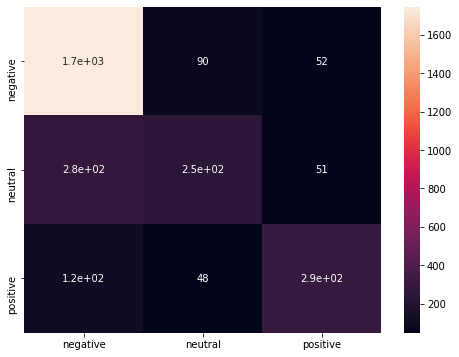
\includegraphics[width=175pt]{graphics/heatmap_LSTM_6_slow.png}
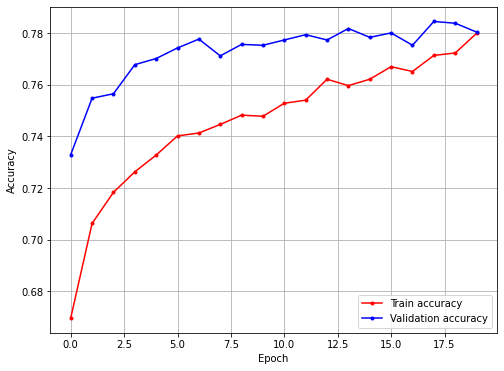
\includegraphics[width=175pt]{graphics/accuracy_LSTM_6_slow.png}
\end{center}
Sieć prawidłowo rozpoznaje większość tweetów o sentymencie negatywnym: około 1700 było prawdziwie negatywne, a 400 fałszywie negatywnych (280 neutralnych i 120 pozytywnych). Jednak w przypadku tweetów neutralnych czy pozytywnych, prezycja spada - na rozpoznane około 390 neutralnych, tylko 250 było neutralne, a 390 rozpoznanych pozytywnie, tylko 290 było pozytywne. Ogólnie dokładność przy 20 epokach uczenia wyniosła 78 \%.
\\ \\
 {\bf Sieć dla 10 słów tweetów}
\begin{center}
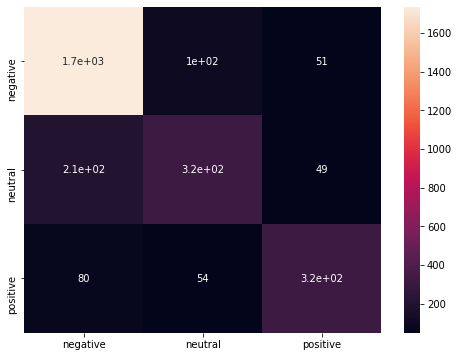
\includegraphics[width=175pt]{graphics/heatmap_LSTM_10_slow.png}
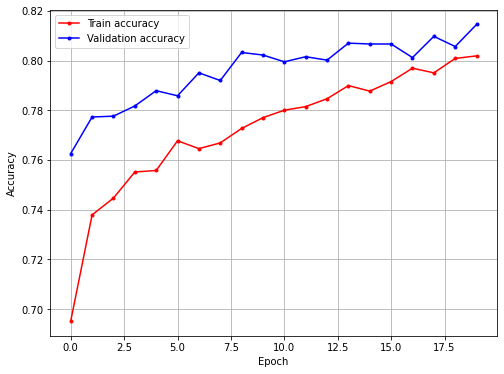
\includegraphics[width=175pt]{graphics/accuracy_LSTM_10_slow.png}
\end{center}
\\ \\
Po zwiększeniu ilości słów branych pod uwagę z 6 na 10, dokładność wzrosła do 81,5 \%. Przypadki pozytywne zaczęły być częściej prawidłowo rozpoznawane (320 zamiast 290), tak samo jak przypadki neutralne (wzrost z 250 do 320). Tym samym dokładność rozpoznanych przypadków negatywnych jest większa (wzrost z 81 \% do 85 \%)
\newpage

 {\bf Sieć dla 20 słów tweetów}
\begin{center}
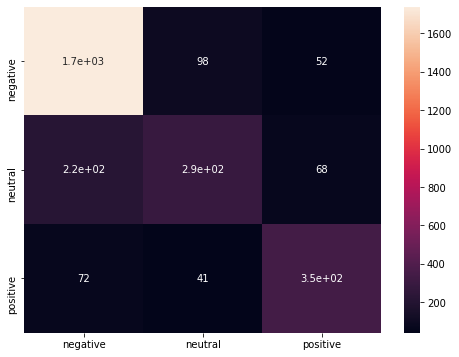
\includegraphics[width=175pt]{graphics/heatmap_LSTM_20_slow.png}
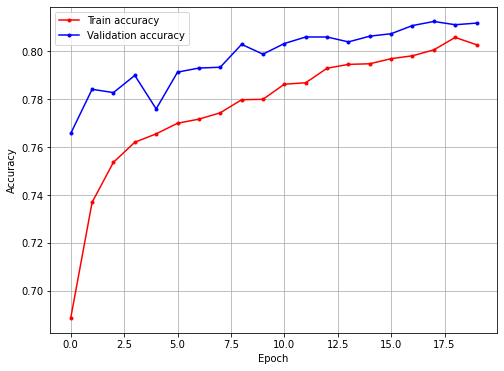
\includegraphics[width=175pt]{graphics/accuracy_LSTM_20_slow.png}
\end{center}
\\ \\
Po zwiększeniu ilości słów branych pod uwagę z 10 na 20, dokładność jest praktycznie taka sama jak wcześniej. Odrobinę zwiększyła się ilość prawidłowo rozpoznawanych przypadków pozytywnych (350 zamiast 320), jednak pogorszyło się rozpoznawanie przypadków neutralnych (spadek z 320 do 290). Przypadki negatywne są dalej rozpoznawane w podobnej ilości, a dokładność pozostała bez zmian - wciąż  85 \% .


\subsection{Sieć LSTM z czterema warstwami}
\begin{center}
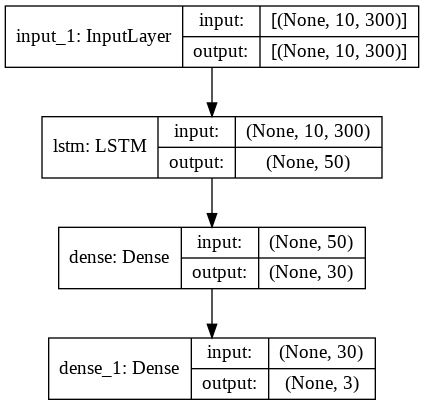
\includegraphics[width=200pt]{graphics/model_LSTM_4_warstwy_10.png}
\end{center}
Druga wersja sieci LSTM zawiera dodatkową warstwę gęstą posiadającą 50 neuronów. Pozostałe warstwy sieci pozostawliśmy bez zmian. Biorąc pod uwagę wyniki poprzednich sieci - gdzie najlepiej spisała się sieć dla 10 pierwszych słów tweeta, wszystkie następne wersje sieci testujemy tylko dla tego rozmiaru danych wejściowych. Tę sieć również trenujemy przez 20 epok.

\subsection{Wyniki treningu sieci LSTM z czterema warstwami}
\begin{center}
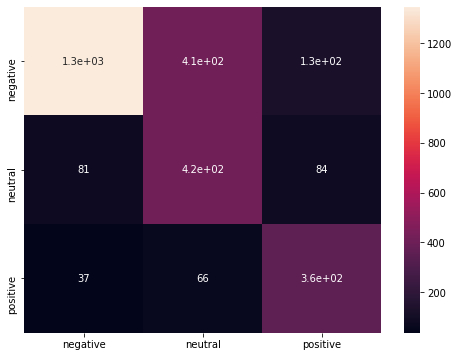
\includegraphics[width=175pt]{graphics/heatmap_LSTM_4_10_slow.png}
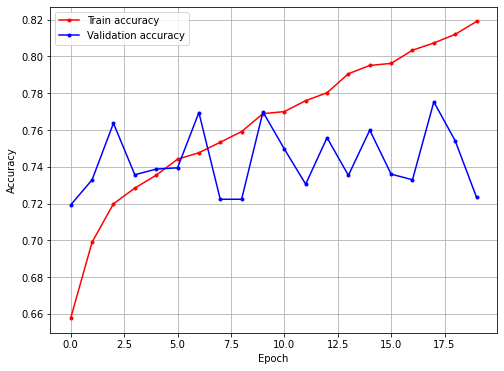
\includegraphics[width=175pt]{graphics/accuracy_LSTM_4_10_slow.png}
\end{center}
Trenowanie sieci LSTM z czterema warstwami po 20 epokach daje aż 92 \% dokładność na zbiorze trenującym, jednak dokładność na zbiorze testującym wynosi od 72 do 77 \% już od pierwszych epok. Wynika z tego, że sieć jest przetrenowana. W porównaniu do sieci LSTM z trzema warstwami, obecna sieć dużo rzadziej przewiduje klasę negatywną (jedynie 1400 zamiast ≈2100), jednak prezycja wzrasta aż do 92 \%. Odbija się to za to na klasie neutralnej: tym razem jest więcej prawidłowych rozpoznań klasy neutralnej (420), jednak pojawiło się też dużo (410) błędnych rozpoznań klasy negatywnej - dokładność spadła . W przypadku klasy pozytywnej wystąpiła podobna sytuacja: jest więcej prawidłowych rozpoznań (360 zamiast 350), jednak nieprawidłowych rozpoznań jest 214 zamiast 120 - dokładność spadła z 83 na 63 \%.

\subsection{Sieć GRU z trzema warstwami}
\begin{center}
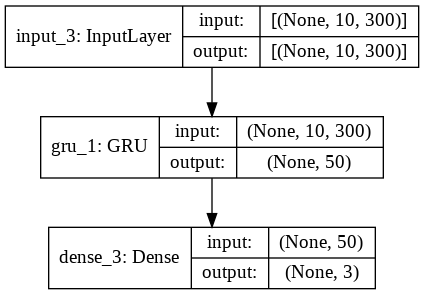
\includegraphics[width=200pt]{graphics/model_GRU_3_warstwy_10.png}
\end{center}
Po sprawdzeniu jak radzą sobie z danymi sieci oparte o jednostki rekurencyjne LSTM, postanowiliśmy powtórzyć eksperymenty dla sieci opartych o drugi rodzaj jednostek rekurencyjnych, czyli GRU. Na początek sprawdzamy wersję z 3 warstwami, w tym wartwą 50 neuronów typu GRU. Tę sieć trenujemy przez 50 epok.

\subsection{Wyniki treningu sieci GRU z trzema warstwami}
\begin{center}
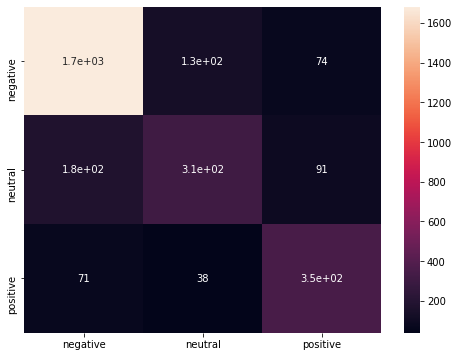
\includegraphics[width=175pt]{graphics/heatmap_GRU_10_slow.png}
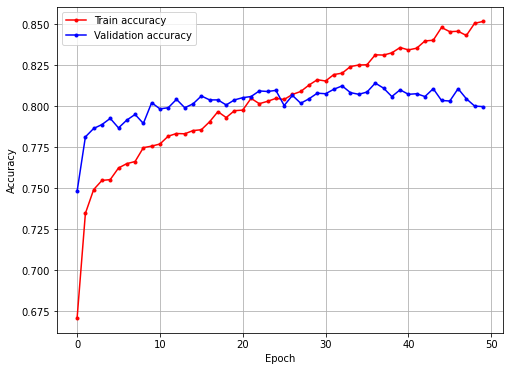
\includegraphics[width=175pt]{graphics/accuracy_GRU_10_slow.png}
\end{center}
Trenowanie sieci GRU z trzema warstwami daje najlepsze wyniki już koło 25 epoki (z 50 epok które przeprowadziliśmy), później dochodzi do przetrenowania. Dokładność wynosi około 81 \%. Najlepiej rozpoznawane są rekordy negatywne - 87 \% precyzja. Rekordy neutralne - 65 \% precyzja. Rekordy pozytywne - 68 \% precyzja.

\subsection{Sieć GRU z czterema warstwami}
\begin{center}
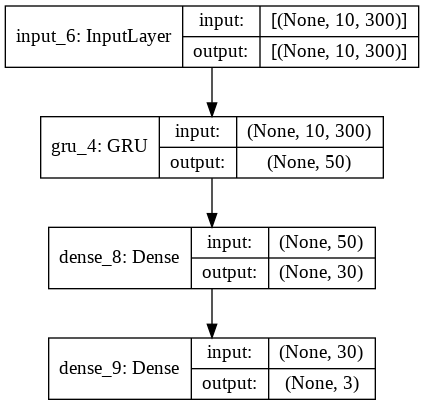
\includegraphics[width=200pt]{graphics/model_GRU_4_warstwy_10.png}
\end{center}
Również dla jednostek GRU druga wersja sieci zawiera dodatkową warstwę gęstą posiadającą 50 neuronów. Pozostałe warstwy sieci pozostawliśmy bez zmian. Tę sieć również trenujemy przez 50 epok.

\subsection{Wyniki treningu sieci GRU z czterema warstwami}
\begin{center}
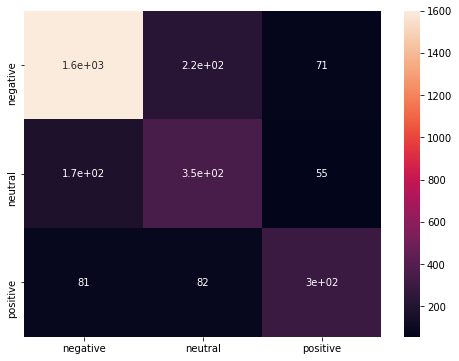
\includegraphics[width=175pt]{graphics/heatmap_GRU_4_10_slow.png}
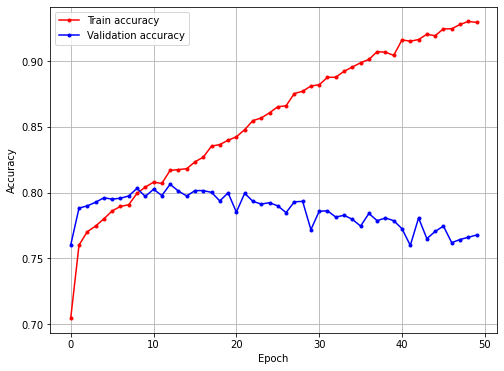
\includegraphics[width=175pt]{graphics/accuracy_GRU_4_10_slow.png}
\end{center}
Jeśli ilość warstw w sieci GRU zwiększymy do czterech, to dokładność na zbiorze trenującym rośnie od 70, aż do 94 \%, jednak na zbiorze testującym osiąga maksymalnie 80 \% przy 10 epokach (podobny wynik jak poprzednio), a później spada do 76 \% - dochodzi do przetrenowania jeszcze szybciej niż przy trzech warstwach (~25 epok). Niewielka ilość rekordów sklasyfikowanych uprzednio jako negatywne, została teraz sklasyfikowana jako neutralne. Dodatkowo część prawidłowych klasyfikacji pozytywnych, zostało teraz błędnie sklasyfikowane jako negatywne lub neutralne (spadek z 350 do 300 prawidłowych)

\newpage
\subsection{Optymalizacja najlepszej z sieci}

Z powyższych testów wynika, że najlepszą skuteczność w stosunku do czasu treningu uzyskał 3 warstwowy model LSTM z wejściami na 10 słów na przykład uczący. Postanowiliśmy zatem dostroić jego parametry. Ze względu na długi czas treningu modelu, postanowiśmy wyszukiwać optymalne parametry po kolei, a nie testować ich różne kombinacje.
\subsubsection{Na początek sprawdziliśmy optymalną wartość parametru dropout warstwy LSTM (testujemy wartości od 10\% do 50\% co 10\%)}
\\ \\
\begin{center}
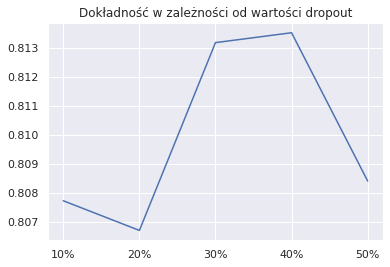
\includegraphics[width=200pt]{graphics/accuracy_dropout.png}
\end{center}
Jak widać na powyższym wykresie, najlepszą dokładność na zbiorze testującym osiąga się przy 40\% poziomie dropoutów. Podobne wyniki osiągane są też przy poziomie 30\% dropotów. Dla pozostałych testowanych wartości osiągana dokładność jest o 0.5-0.7\% niższa. W związku z tym do dalszych eksperymentów wybieramy sieć z poziomem dropout 40\% .

\subsubsection{Następnie sprawdziliśmy optymalną ilość neuronów w warstwie LSTM (od 30 do 100 neuronów co 10 neuronów)}
\\ \\
\begin{center}
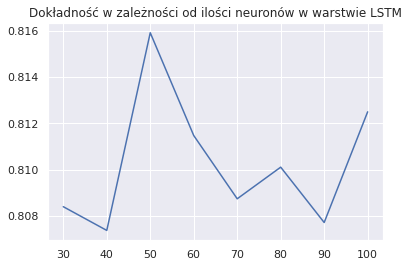
\includegraphics[width=200pt]{graphics/accuracy_neurons.png}
\end{center}
Jeśli chodzi o wpływ ilości neuronów w warstwie rekurencyjnej na dokładność sieci względem danych testujących to z naszych testów wyraźnie wynika, że najlepsze rezultaty są osiągane przy 50 neuronach rekurencyjnych - osiagana dokładność to około 81.6\% . Pozostałe wersje sieci są gorsze o 0.4-0.8\% .  Widać również wzrost dokładności przy zastosowaniu 100 neuronów, jednak nawet tamten wynik jest gorszy niż przy 50 neuronach. W związku z tym do dalszych eksperymentów wybieramy sieć z 50 neuronami rekurencyjnymi.

\subsubsection{Na koniec sprawdziliśmy, który optymalizator sieci będzie najlepszy (sgd, rmsprop, adam)}
\\ \\
\begin{center}
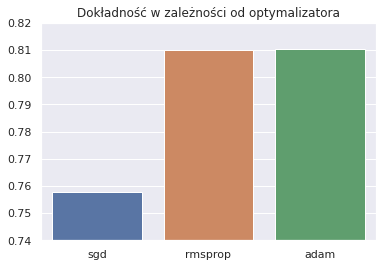
\includegraphics[width=200pt]{graphics/accuracy_optimizer.png}
\end{center}
Jak widać na wykresie kolumnowym, sieć z optymalizatorem sgd osiągnęła dokładność około 76\% co jest jednak wynikiem o około 5\% słabszym od optymalizatorów adam i rmsprop. Te dwa optymalizatory spisały się praktycznie identycznie - różnica na korzyść optymalizatora adam wynosi zaledwie około 0.03\% . W takim przypadku wybieramy jednak optymalizator adam.

\subsection{Najlepszy model}
Najlepszy model posiada 3 warstwy: warstwę wejściową na 10 pierwszych słów tweeta, 50 jednostek LSTM z dropoutem 40 \%, warstwę wyjściową oraz używa optymalizatora Adam. Poniżej wyniki ostatniego treningu najlepszego modelu:
\begin{center}
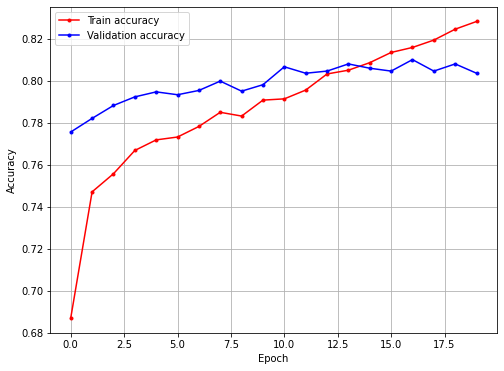
\includegraphics[width=175pt]{graphics/best_model_accuracy.png}
\end{center}

Najlepsze wyniki zostają osiągnięte przy około 17 epokach uczenia: parametr validation accuracy osiąga 81 \%.


\chapter{Podsumowanie}
W projekcie sprawdziliśmy kilka metod uczenia nadzorowanego dla zadania klasyfikacji - wbudowany model w bibliotece fastText oraz sieci rekurencyjne z jednostkami LSTM i GRU z różną ilością warstw i hiperparametrami. Najlepszy okazał się model sieci neuronowej z 3 warstwami, posiadający 50 jednostek LSTM. Uzyskał on dokładność około 81\% względem zbioru testowego. Model ten przyjmował na wejściu 10 pierwszych słów tweeta zakodowanych jako wektory 300 wymiarowe w dziedzinie semantycznej słów (word embedding). Model wbudowany w bibliotekę fastText osiągnął precyzję około 75\% względem zbioru testowego, czyli mniejszą niż nasz model specjalizowany - jednak jest on szybki w użyciu i nie wymaga sprawdzania różnych architektur sieci. Wśród błędnie dopasowanych tweetów najlepszego modelu wiele było bardzo krótkich, przez co trudnych do klasyfikacji nawet dla człowieka. Średnia długość tweeta błędnie dopasowanego wynosiła 97 znaków, a poprawnie dopasowanego 106 znaków co potwierdza, że długość tweeta miała wpływ na dokładność. Innym czynnikiem była duża ilość emotikonów oraz znaków nie pochodzących z alfabetu angielskiego jak na przykład '@' co również utrudniało klasyfikację. Podsumowując nasz model osiągnął bardzo dobry wynik, biorąc pod uwagę jakość użytych danych.


\begin{appendices}
\chapter{Kod programu}
\begin{spverbatim}
import re
import nltk
import fasttext
import numpy as np
import pandas as pd
import seaborn as sns
import matplotlib.pyplot as plt

from keras.models import Sequential
from keras import layers
from keras import regularizers
from keras.utils.vis_utils import plot_model
from sklearn.utils.class_weight import compute_class_weight

from sklearn.model_selection import train_test_split
from sklearn.metrics import confusion_matrix

from nltk.corpus import stopwords
from numpy import save
from numpy import asarray
from numpy import load

#fastText - Wbudowany model

models_precision = []
for i in range(1,5):
    epochs = []
    for j in range(5,30,5):
        model = fasttext.train_supervised("/content/drive/MyDrive/NLP_SI/tweets_2_train.txt", epoch=j, wordNgrams=i)
        d = model.test_label("/content/drive/MyDrive/NLP_SI/tweets_2_test.txt")
        epochs.append({label: value['precision'] for label, value in d.items()})
    models_precision.append(epochs)

plots_data = [pd.DataFrame(precision) for precision in models_precision]

for plot_data in plots_data:
    plot_data.index = range(5,30,5)
    plot_data['mean'] = plot_data.mean(axis=1)

f, ax = plt.subplots(2, 2, figsize=(20,10))
for i in range(4):
    sns.lineplot(data=plots_data[i], legend='brief', ax=ax[i//2][i%2]).set(xlim=(5,32))
    ax[i//2][i%2].legend([label.replace("__label__", "") for label in plots_data[i].columns], loc="lower right")
    ax[i//2][i%2].set_title(f"Ngramy od 1 do {i+1}")
plt.show()

#Przygotowanie danych do uczenia sieci neuronowych

tweets = pd.read_csv(r"/content/drive/MyDrive/NLP_SI/Tweets_1.csv")
tweets_test = tweets.sample(frac=0.2, random_state=42)
tweets_train = tweets[~tweets.index.isin(tweets_test.index)]

nltk.download('stopwords')
ft = fasttext.load_model('cc.en.300.bin')

pattern = re.compile('[^A-Za-z]+')

tweets_train_vectors = []
total_difference = 0
total_length_initial = 0
for x in tweets_train[['text']].values:
  try:
    x = x[0].replace(r"\n", " ").replace(r"\r", " ")
    x_list = x.split(" ")
    total_length_initial += len(x_list)
    filtered_words = [pattern.sub('', word) for word in x_list if word not in stopwords.words('english')]
    filtered_words = [x for idx, x in enumerate(filtered_words) if x.strip() and idx != 0]
    total_difference += len(x_list) - len(filtered_words)
    tweets_train_vectors.append([ft.get_word_vector(x) for x in filtered_words])
  except ValueError:
    print(x)

tweets_test_vectors = []
for x in tweets_test[['text']].values:
  try:
    x = x[0].replace(r"\n", " ").replace(r"\r", " ")
    x_list = x.split(" ")
    total_length_initial += len(x_list)
    filtered_words = [pattern.sub('', word) for word in x_list if word not in stopwords.words('english')]
    filtered_words = [x for idx, x in enumerate(filtered_words) if x.strip() and idx != 0]
    total_difference += len(x_list) - len(filtered_words)
    tweets_test_vectors.append([ft.get_word_vector(x) for x in filtered_words])
  except ValueError:
    print(x)

total_length = 0
for statement in tweets_train_vectors:
  total_length += len(statement)
print(f"Average sentence length {round(total_length/len(tweets_train_vectors), 2)}")
print(f"Percent of used words {round((1 - total_difference/total_length_initial)*100, 2)}%")

tweets_final_vectors = {'test':{6: [], 10: [], 20: []}, 'train':{6: [], 10: [], 20: []}}
def compute_vectors(tweets_vectors, kind):
  for i in (6, 10, 20):
    zero_vectors = 0
    shrinked_vectors = 0
    for statement in tweets_vectors:
      if len(statement) < i:
        tweets_final_vectors[kind][i].append(np.array(statement+[[0] * 300]*(i-len(statement))))
        zero_vectors += i-len(statement)
      else:
        tweets_final_vectors[kind][i].append(np.array(statement[:i]))
        shrinked_vectors += len(statement) - i
    print(f"Zero vectors {zero_vectors/len(tweets_vectors)} for statement")
    print(f"Shrinked vectors {shrinked_vectors/len(tweets_vectors)} for statement")
    print()

compute_vectors(tweets_train_vectors, 'train')
compute_vectors(tweets_test_vectors, 'test')

for key in tweets_final_vectors.keys():
  for i in tweets_final_vectors[key].keys():
    data = asarray(tweets_train_vectors_3)
    save(f'/content/drive/MyDrive/NLP_SI/data_{key}_ext_{i}.npy', data)

base_path = '/content/drive/MyDrive/NLP_SI/'
paths = {kind: [f'data_{kind}_ext.npy', f'data_{kind}_ext_10.npy', f'data_{kind}_ext_20.npy'] for kind in ('train', 'test')}
data = [load(base_path+file_path) for file_path in paths['train']]
data_test = [load(base_path+file_path) for file_path in paths['test']]
tweets = pd.read_csv(r"/content/drive/MyDrive/NLP_SI/Tweets_1.csv")
tweets_test = tweets.sample(frac=0.2, random_state=42)
tweets_train = tweets[~tweets.index.isin(tweets_test.index)]

tweets_train_y = tweets_train.airline_sentiment.map({'negative': 0, 'neutral': 1, 'positive': 2}).values
tweets_test_y = tweets_test.airline_sentiment.map({'negative': 0, 'neutral': 1, 'positive': 2}).values
data_y = np.zeros((tweets_train_y.size, tweets_train_y.max()+1))
data_y[np.arange(tweets_train_y.size),tweets_train_y] = 1
data_test_y = np.zeros((tweets_test_y.size, tweets_test_y.max()+1))
data_test_y[np.arange(tweets_test_y.size),tweets_test_y] = 1

#Trenowanie sieci LSTM

models = []

for i in (6, 10, 20):
  model = Sequential()
  model.add(layers.InputLayer(input_shape=(i,300)))
  model.add(layers.LSTM(50,dropout=0.5))
  model.add(layers.Dense(3,activation='softmax'))
  model.compile(optimizer='rmsprop',loss='categorical_crossentropy', metrics=['accuracy'])
  models.append(model)

for i, model in zip((6, 10, 20), models):
  plot_model(model, to_file=f'model_LSTM_3_warstwy_{i}.png', show_shapes=True, show_layer_names=True)

models_history = []
for i, (X, X_test, model) in enumerate(zip(data, data_test, models)):
  print(f'Model {i}')
  models_history.append(model.fit(X, data_y, epochs=20, validation_data=(X_test, data_test_y), verbose=True))
  print()

for i, X, X_test, model, run_history in zip((6, 10, 20), data, data_test, models, models_history):
  print(f'\nModel dla pierwszych {i} słów tweeta\n')
  p = model.predict(X_test)
  y_pred = (p == p.max(axis=1)[:,None]).astype(float)
  sns.heatmap(confusion_matrix(data_test_y.argmax(axis=1), y_pred.argmax(axis=1)), annot=True, xticklabels=['negative', 'neutral', 'positive'], yticklabels=['negative', 'neutral', 'positive'])
  plt.show()
  print()
  plt.rcParams['figure.figsize'] = (8.0, 6.0)
  plt.plot(run_history.history["accuracy"],'r', marker='.', label="Train accuracy")
  plt.plot(run_history.history["val_accuracy"],'b', marker='.', label="Validation accuracy")
  plt.legend()
  plt.xlabel('Epoch'), plt.ylabel('Accuracy')
  plt.grid()
  plt.show()

y_integers = np.argmax(data_y, axis=1)
class_weights = compute_class_weight('balanced', np.unique(y_integers), y_integers)
d_class_weights = dict(enumerate(class_weights))

deep_model = Sequential()
deep_model.add(layers.InputLayer(input_shape=(10,300)))
deep_model.add(layers.LSTM(50,dropout=0.2))
deep_model.add(layers.Dense(30))
deep_model.add(layers.Dense(3,activation='softmax'))
deep_model.compile(optimizer='rmsprop',loss='categorical_crossentropy', metrics=['accuracy'])

plot_model(deep_model, to_file='model_LSTM_4_warstwy_10.png', show_shapes=True, show_layer_names=True)

deep_model_history = deep_model.fit(data[1], data_y, epochs=20, validation_data=(data_test[1], data_test_y),class_weight=d_class_weights, verbose=True)

print(f'\nModel dla pierwszych 10 słów tweeta z warstwą gęstą i wagami klas\n')
p = deep_model.predict(data_test[1])
y_pred = (p == p.max(axis=1)[:,None]).astype(float)
sns.heatmap(confusion_matrix(data_test_y.argmax(axis=1), y_pred.argmax(axis=1)), annot=True, xticklabels=['negative', 'neutral', 'positive'], yticklabels=['negative', 'neutral', 'positive'])
plt.show()
print()
plt.rcParams['figure.figsize'] = (8.0, 6.0)
plt.plot(deep_model_history.history["accuracy"],'r', marker='.', label="Train accuracy")
plt.plot(deep_model_history.history["val_accuracy"],'b', marker='.', label="Validation accuracy")
plt.legend()
plt.xlabel('Epoch'), plt.ylabel('Accuracy')
plt.grid()
plt.show()

deep_model_history = deep_model.fit(data[1], data_y, epochs=20, validation_data=(data_test[1], data_test_y), verbose=True)

#Trenowanie sieci GRU

gru_model = Sequential()
gru_model.add(layers.InputLayer(input_shape=(10,300)))
gru_model.add(layers.GRU(50,dropout=0.5))
gru_model.add(layers.Dense(3,activation='softmax'))
gru_model.compile(optimizer='rmsprop',loss='categorical_crossentropy', metrics=['accuracy'])

plot_model(gru_model, to_file='model_GRU_3_warstwy_10.png', show_shapes=True, show_layer_names=True)

deep_model_history = gru_model.fit(data[1], data_y, epochs=50, validation_data=(data_test[1], data_test_y), verbose=True)

print(f'\nModel dla pierwszych 10 słów tweeta z jednostkami GRU\n')
p = gru_model.predict(data_test[1])
y_pred = (p == p.max(axis=1)[:,None]).astype(float)
sns.heatmap(confusion_matrix(data_test_y.argmax(axis=1), y_pred.argmax(axis=1)), annot=True, xticklabels=['negative', 'neutral', 'positive'], yticklabels=['negative', 'neutral', 'positive'])
plt.show()
print()
plt.rcParams['figure.figsize'] = (8.0, 6.0)
plt.plot(deep_model_history.history["accuracy"],'r', marker='.', label="Train accuracy")
plt.plot(deep_model_history.history["val_accuracy"],'b', marker='.', label="Validation accuracy")
plt.legend()
plt.xlabel('Epoch'), plt.ylabel('Accuracy')
plt.grid()
plt.show()

gru_model = Sequential()
gru_model.add(layers.InputLayer(input_shape=(10,300)))
gru_model.add(layers.GRU(50,dropout=0.2))
gru_model.add(layers.Dense(30))
gru_model.add(layers.Dense(3,activation='softmax'))
gru_model.compile(optimizer='rmsprop',loss='categorical_crossentropy', metrics=['accuracy'])

plot_model(gru_model, to_file='model_GRU_4_warstwy_10.png', show_shapes=True, show_layer_names=True)

deep_model_history = gru_model.fit(data[1], data_y, epochs=50, validation_data=(data_test[1], data_test_y), verbose=True)

print(f'\nModel dla pierwszych 10 słów tweeta 4 warstwowy z jednostkami GRU\n')
p = gru_model.predict(data_test[1])
y_pred = (p == p.max(axis=1)[:,None]).astype(float)
sns.heatmap(confusion_matrix(data_test_y.argmax(axis=1), y_pred.argmax(axis=1)), annot=True, xticklabels=['negative', 'neutral', 'positive'], yticklabels=['negative', 'neutral', 'positive'])
plt.show()
print()
plt.rcParams['figure.figsize'] = (8.0, 6.0)
plt.plot(deep_model_history.history["accuracy"],'r', marker='.', label="Train accuracy")
plt.plot(deep_model_history.history["val_accuracy"],'b', marker='.', label="Validation accuracy")
plt.legend()
plt.xlabel('Epoch'), plt.ylabel('Accuracy')
plt.grid()
plt.show()

#Optymalizacja najlepszego modelu

model_parameters = {'dropout':{}}

for i in range(1, 6):
  print(f'Testing dropout={i*10}%')
  model = Sequential()
  model.add(layers.InputLayer(input_shape=(10,300)))
  model.add(layers.LSTM(50,dropout=i/10))
  model.add(layers.Dense(3,activation='softmax'))
  model.compile(optimizer='rmsprop',loss='categorical_crossentropy', metrics=['accuracy'])
  run_history = model.fit(data[1], data_y, epochs=20, validation_data=(data_test[1], data_test_y), verbose=True)
  model_parameters['dropout'][i] = max(run_history.history["val_accuracy"])
  print()

model_parameters['neurons_number'] = {}

for i in range(30, 101, 10):
  print(f'Testing number of neurons = {i}')
  model = Sequential()
  model.add(layers.InputLayer(input_shape=(10,300)))
  model.add(layers.LSTM(i,dropout=0.4))
  model.add(layers.Dense(3,activation='softmax'))
  model.compile(optimizer='rmsprop',loss='categorical_crossentropy', metrics=['accuracy'])
  run_history = model.fit(data[1], data_y, epochs=20, validation_data=(data_test[1], data_test_y), verbose=True)
  model_parameters['neurons_number'][i] = max(run_history.history["val_accuracy"])
  print()

model_parameters['optimizer'] = {}

for i in ('sgd', 'rmsprop', 'adam'):
  print(f'Testing optimizer = {i}')
  model = Sequential()
  model.add(layers.InputLayer(input_shape=(10,300)))
  model.add(layers.LSTM(50,dropout=0.4))
  model.add(layers.Dense(3,activation='softmax'))
  model.compile(optimizer=i,loss='categorical_crossentropy', metrics=['accuracy'])
  run_history = model.fit(data[1], data_y, epochs=20, validation_data=(data_test[1], data_test_y), verbose=True)
  model_parameters['optimizer'][i] = max(run_history.history["val_accuracy"])
  print()

sns.set_theme()

g = sns.lineplot(data=model_parameters['dropout'], legend='brief',)
g.set_xticks([x for x in range(1, 6)])
g.set_xticklabels([f"{x*10}%" for x in range(1, 6)])
g.set_title("Dokładność w zależności od wartości dropout")
plt.show()

g = sns.lineplot(data=model_parameters['neurons_number'], legend='brief',)
g.set_xticks([x for x in range(30, 101, 10)])
g.set_title("Dokładność w zależności od ilości neuronów w warstwie LSTM")
plt.show()

keys = list(model_parameters['optimizer'].keys())
vals = [model_parameters['optimizer'][k] for k in keys]
g = sns.barplot(x=keys, y=vals)
plt.ylim(0.74, 0.82)
g.set_title("Dokładność w zależności od optymalizatora")
plt.show()

best_model = Sequential()
best_model.add(layers.InputLayer(input_shape=(10,300)))
best_model.add(layers.LSTM(50,dropout=0.4))
best_model.add(layers.Dense(3,activation='softmax'))
best_model.compile(optimizer='adam',loss='categorical_crossentropy', metrics=['accuracy'])

run_history = best_model.fit(data[1], data_y, epochs=20, validation_data=(data_test[1], data_test_y), verbose=True)

plt.rcParams['figure.figsize'] = (8.0, 6.0)
plt.plot(run_history.history["accuracy"],'r', marker='.', label="Train accuracy")
plt.plot(run_history.history["val_accuracy"],'b', marker='.', label="Validation accuracy")
plt.legend()
plt.xlabel('Epoch'), plt.ylabel('Accuracy')
plt.grid()
plt.show()

plot_model(best_model, to_file='best_model.png', show_shapes=True, show_layer_names=True)

probabilities = []
predicted = best_model.predict(data_test[1])
for i, idx in enumerate(np.argmax(predicted, axis=-1)):
  probabilities.append(predicted[i][idx])

tweets_test['predicted_sentiment'] = np.argmax(best_model.predict(data_test[1]), axis=-1)
tweets_test['predicted_sentiment'] = tweets_test['predicted_sentiment'].map({0: 'negative', 1: 'neutral', 2: 'positive'})
tweets_test['predicted_confidence'] = probabilities

tweets_test_errors = tweets_test.query('airline_sentiment != predicted_sentiment')

tweets_test_correct = tweets_test.query('airline_sentiment == predicted_sentiment')

print(f'Correct average length {round(tweets_test_errors.text.str.len().sum() / len(tweets_test_errors), 2)}, errors average length {round(tweets_test_correct.text.str.len().sum() / len(tweets_test_correct), 2)}')

tweets_test_errors.sort_values(by="text", key=lambda x: x.str.len()).head(20)

pd.set_option('max_colwidth', -1)
tweets_test_errors.sort_values(by="predicted_confidence").head(20)

\end{spverbatim}
\end{appendices}

\end{document}